\documentclass[12pt,letterpaper]{ntdhw}


\usepackage{ntdmath}

\title{Project 1: Regular Languages and Pursuit-Evasion}
\author{CSCI 561}

\rhead{Names: Luke Beukelman, Ben Breisch, Luc Lafave, Adam Thistlewood}

%\keytrue

\begin{document}
\pagestyle{fancyplain}

\maketitle
\thispagestyle{fancyplain}
%\clearpage



\section*{Application: Text Processing with Grep}

\begin{quote}
  \emph{\texttt{grep} is a unix utility that searches text for lines
    matching a regular expression.}
\end{quote}

\begin{enumerate}
  \item \textbf{Using Grep:} Use the standard unix (or GNU)
  \texttt{grep} and the implementation in this project to search the
  starter code for all \texttt{TODO}s.
  \begin{figure}[htp]
    \centering
    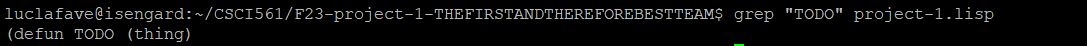
\includegraphics[width=17cm]{unixGrep.JPG}
    \caption{Unix Grep}
  \end{figure}
  \begin{figure}[htp]
    \centering
    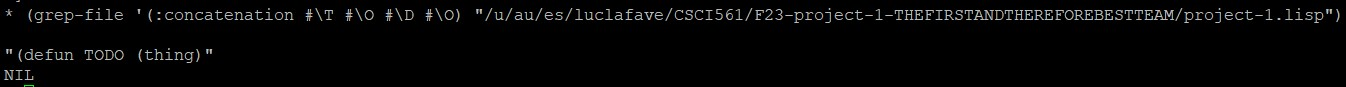
\includegraphics[width=17cm]{trivialgrep.jpg}
    \caption{Trivial Grep}
  \end{figure}
  

  \item \textbf{NFA vs. DFA Simulation:} The original grep utility (as
  written by Ken Thompson) converted the provided regular expression
  to an NFA and then simulated the NFA on the input text.  Why would
  Thompson have used NFA simulation instead of DFA simulation?
  \par \textbf{Answer 2:} I would assume he made this choice for a couple of reasons. The first is I believe that Thompson in 1972 was probably memory constrained, but converting from an NFA to a DFA usually results in a larger DFA. The worst case can be up to $2^n$ nodes more in DFA than NFA  which is exponentially bad in memory constrained environments. Another reason I believe this decision was made is that on top of the memory constraint issues, the time it takes to perform subset construction to convert an NFA to a DFA added plus the time to then perform dfa-simulate was usually not much faster than just preforming Thompson's implementation of nfa-simulate, especially if most nfa's created did not end up being extremely complicated. Additionally, NFAs can handle the OR operator much more efficiently than DFAs because it can explore multiple paths at once. In a DFA, each OR (UNION) operator requires a computationally expensive construction of multiple sub-DFAs for each possible subexpression. For complex expressions with multiple UNION operations, converting from an NFA to a DFA can be extremely space and time expensive.

  \item \textbf{Time Complexity:} To simulate an NFA
  $N=\lmtuple{Q}{\Sigma}{\delta}{q_0}{F}$ on string $\sigma$ using the
  algorithm in the original grep (which is roughly equivalent to the
  NFA simulation algorithm covered in lecture) requires
  $O(|Q|*|\sigma|)$ time. However, many ``regex'' engines (including the
  popular implementation in Perl) exhibit worst-case complexity that
  is exponential in $|\sigma|$.

  \begin{enumerate}
    \item Prove that NFA simulation is possible in $O(|Q|*|\sigma|)$
      time.%
      \par \textbf{Answer 3a:} Using Thompson's implementation of NFA simulate it is possible to perform the algorithm in the runtime of $O(|Q|*|\sigma|)$. 
      \begin{enumerate}
          \item[1.] Initialize two lists a current states list and a list of next states.
          \item[2.]  Fill current states list with the start state.
          \item[3.] For each character in the string loop through the current states and find the next states add to list. If one next state is an accept state break and print string in language. 
          \item[4.] Set current states list to be next states list then move to next string. If no new next states exist break and print string not in language.
          \item[5.] This is time complexity of $|\sigma| * |Q|$ because you go through length of string and for each character you loop through each state. The worst case can be looping through all the states in the NFA which is $|Q|$. This means that it could end up taking  $|\sigma| * |Q|$.
      \end{enumerate}

    \item Why is there such a difference in performance between
      Thompson's grep and some other ``regex'' engines?
      \par \textbf{Answer 3b:} The reasons there is a difference in the performance between Thompson's grep and other regex engines like perl is because some regex engines like perl use backtracking in their implementations on nfa simulate while Thompson's uses a smarter approach of perfect guessing which allows the fa to be in multiple states at once. Thompson's approach only tracks reachable states from current states, not the paths themselves. If the string does not belong it will quit as soon as there are no possible next states to transition using the current character of the string being simulated on NFA. In the perl approach it tries one path and if that fails to reach the accept state it will try the next path. And in the instance that a string does not belong in the language the perl method of NFA simulate will result in all possible execution paths being tried before failing. This backtracking simple recursive method is exponential in its runtime in terms of $\sigma$. 
  \end{enumerate}




\end{enumerate}

\clearpage
\section*{Application: Discrete Event Systems Model of Pursuit-Evasion}

\begin{figure}[b]
  \centering
  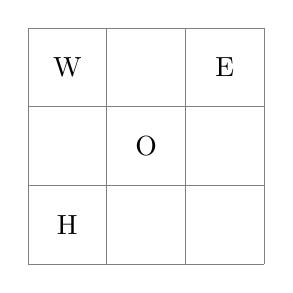
\begin{tikzpicture}
    \draw[step=1cm,gray,very thin,xshift=.5cm,yshift=.5cm] (-1,-1) grid (2,2);
    \node at (0cm,2cm) {W};
    \node at (0cm,0cm) {H};
    \node at (1cm,1cm) {O};
    \node at (2cm,2cm) {E};
  \end{tikzpicture}
  \caption{Example wumpus-world map.  W represents the initial
    location of the wumpus.  H represents the initial location of the
    human.  E represents the escape location.  O represents an
    obstacle that neither the human nor wumpus can move into.}
  \label{fig:map}
\end{figure}

\begin{quote}

\emph{\emph{Pursuit-evasion games} are scenarios with multiple agents
  where one agent attempts to avoid capture by another.  Consider a
  variation of pursuit-evasion games as follows:}

\begin{itemize}
  \item \it Two agents share a grid environment: a human (evader) and wumpus
  (pursuer).
  \item \it The human and wumpus alternate moves on the grid.  The
  wumpus moves each turn up, down, left or right.  The human can move
  up, down, left, right, or remain in place.  You may assume that the
  human moves first.
  \item \it If the wumpus and human ever occupy the same grid cell,
  the wumpus eats the human.
  \item \it If the human reaches a designated grid cell, they escape.
\end{itemize}

\emph{Answer the following questions using your implementation of finite
automata operations for support.}

\end{quote}

\begin{enumerate}

  \item For the map in \autoref{fig:map}, construct a discrete event
  system model.  Assume that the human's movements are controllable
  and that the wumpus's movements are not controllable.
  
To start, we create finite automatons that describe all possible moves for the wumpus and the human separately. We omit locations that either the wumpus or the human cannot inhabit because of an obstacle. Our discrete event system model is the product finite automaton of each player's respective FA. In the individual FAs, each transition between states has an associated symbol that describes what happens when that edge is taken. The list below shows each possible transition.
\begin{enumerate}
    \item human\_up
    \item human\_down
    \item human\_left
    \item human\_right
    \item human\_stay
    \item wumpus\_up
    \item wumpus\_down
    \item wumpus\_left
    \item wumpus\_right
    
\end{enumerate}The figure below shows the graphvis representation of the finite automaton for this map.

\begin{center}
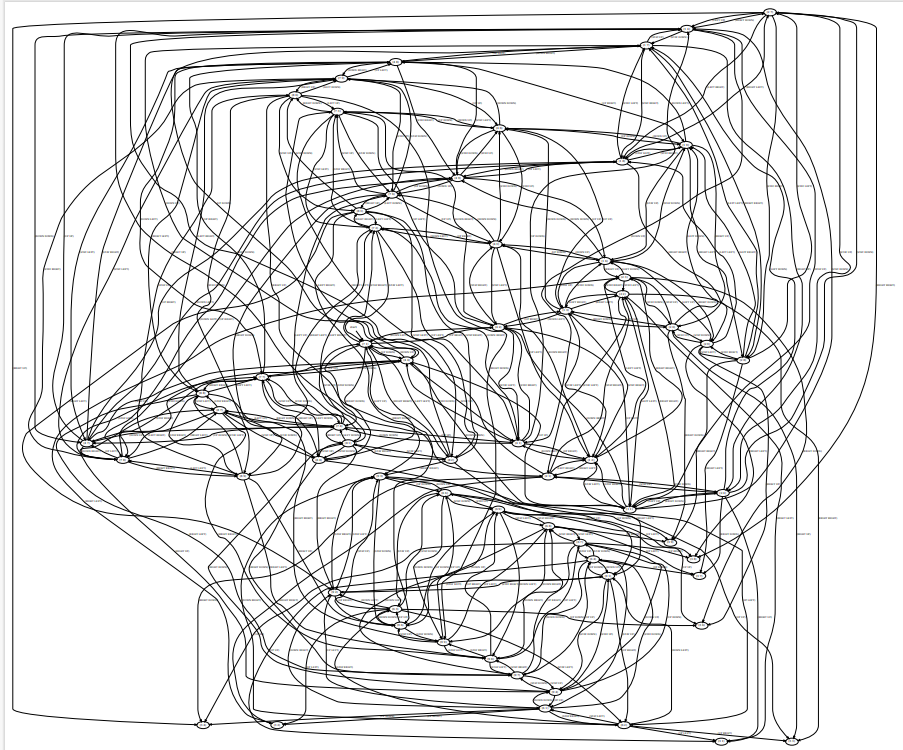
\includegraphics[scale=0.5]{Q2_graphviz.png}
\end{center}

  \item For your DES model of \autoref{fig:map}, construct a specification
  for the human to avoid the wumpus and escape.
  \begin{enumerate}
    \item Can the human guarantee to avoid being eaten, no matter what
    the wumpus does?  Prove yes or no via automata operations.
    
    Given the individual finite automata for the states that the human and wumpus can be in, the product dfa of those two finite automatons describe the entire state space of the game. Given the product dfa, if there exists a path to a state where the human is at the location of the escape point and there is never a state in which the location of the wumpus and the human are the same along that path, we can guarantee that the human can avoid being eaten no matter what the wumpus does.
    \item Can the human always to escape in finite time (fixed
    number of steps), no matter what the wumpus does?  Prove yes or
    no.

    Given the product dfa of the individual finite automatons for the human and the wumpus, we can inspect the dfa in order to guarantee that the human will always escape in finite time. First we start by searching the DES model for a path to an accept state without any intermediate states where the location of the human and the wumpus are the same. Along all of these paths we must also check for cycles, which would mean the human could escape in infinite time.  If any of these cycles exist, we conclude that the human cannot always escape in finite time.
  \end{enumerate}

  \item Design a map where the wumpus can always eat the human and
  prove via a DES model that this is the case.

  The map below describes a world where the wumpus will always be able to eat the human.
  \begin{center}
  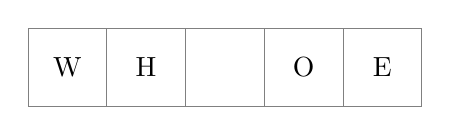
\begin{tikzpicture}
    \draw[step=1cm,gray,very thin,xshift=.5cm,yshift=.5cm] (-1,-1) grid (4,0);
    \node at (0cm,0cm) {W};
    \node at (1cm,0cm) {H};
    \node at (3cm,0cm) {O};
    \node at (4cm,0cm) {E};
  \end{tikzpicture}
  \label{fig:map3}
\end{center}

The DES model below follows the same setup as Q1 above. As you can see, there are no accept states in the DES model, which is a product DFA of the FA for the wumpus and the human. Because there are no accept states, the wumpus will always eat the human, no matter what the human does.
\begin{center}
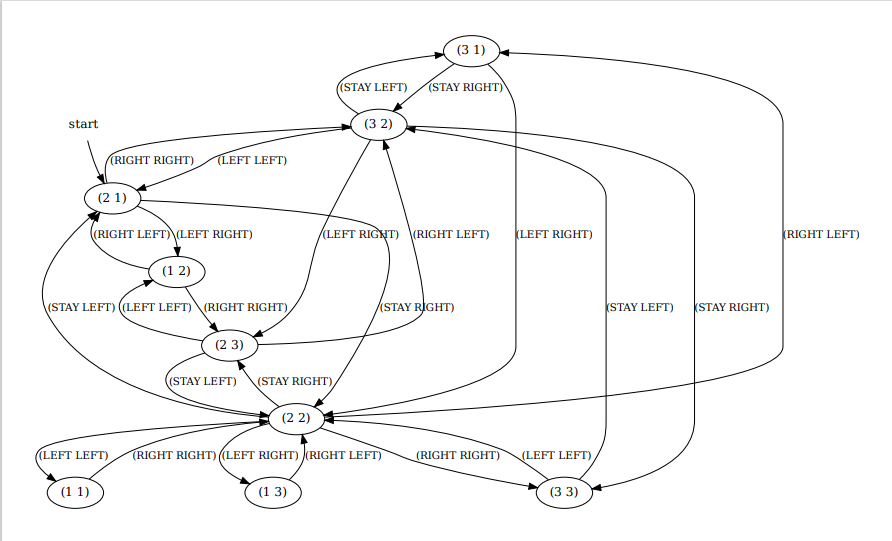
\includegraphics[scale=0.5]{Q3_graphviz.png}
\end{center}
  \item Design a map where the human can always escape and prove via a
  DES model that this is the case.
  
    The map below describes a world where the wumpus will never be able to eat the human and the human will escape.
    
    \begin{center}
      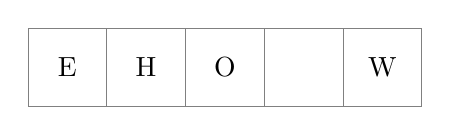
\begin{tikzpicture}
        \draw[step=1cm,gray,very thin,xshift=.5cm,yshift=.5cm] (-1,-1) grid (4,0);
        \node at (0cm,0cm) {E};
        \node at (1cm,0cm) {H};
        \node at (2cm,0cm) {O};
        \node at (4cm,0cm) {W};
      \end{tikzpicture}
      \label{fig:map4}
    \end{center}
As you can see in the DES model below for this scenario, an accept state is always reachable within infinite time. Technically speaking, the human could choose to stay in its current state for infinite time and neither party would win the game but we will assume that the human is sufficiently scared of the wumpus and will move to the escape point.
\begin{center}
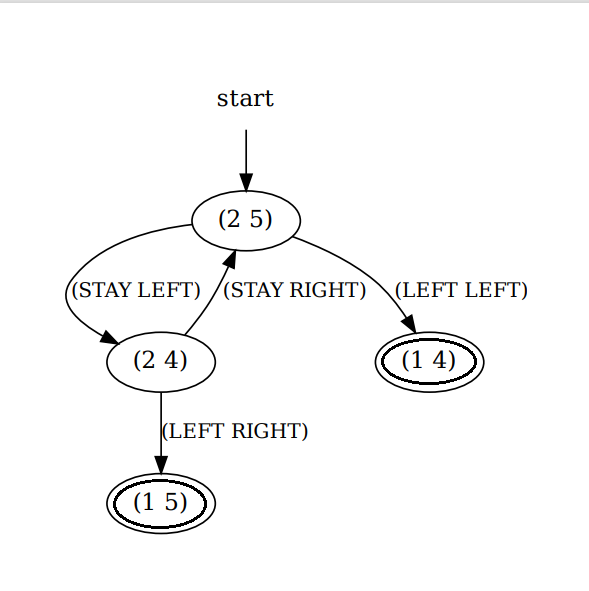
\includegraphics[scale=0.5]{Q4_graphviz.png}
\end{center}
\end{enumerate}
\end{document}


%%% Local Variables:
%%% mode: latex
%%% TeX-master: t
%%% End:
